%!TEX root = ../main.tex
\section{Introduction} 
\label{sec:intro}
Data quality is one of the most significant problems in data management, among which mislabels are a common dirty data type that could directly lead to  low-quality data analysis  and misleading business decisions. Labels are always large-scale and error-prone because they may be crowdsourced from non-experts or collected from web annotations, so it is inevitable to use automatic methods to detect mislabels. However, existing mislabel detection approaches suffer from fair accuracy.


\stitle{Existing Solutions.} Traditional methods~\cite{} rely on the data locality to detect mislabels. For example, in order to whether the label of an instance in a dataset is correct, the typical KNN method~\cite{} checks its neighbors, and if they have inconsistent labels, the instance tends to be mislabeled, otherwise it is a clean one. This type of methods has low detection accuracy because they just consider the local neighbors of each instance rather than the entire dataset. Therefore, to improve the accuracy, machine learning (ML) models are incorporated to help mislabel detection~\cite{} because intuitively,  mislabels definitely have impact on the supervised model training. For instances, ensemble-based methods~\cite{} involve multiple models to train on the entire dataset and check the consistency of the prediction results from these models for each instance. Cleanlab~\cite{} utilizes confident learning to estimate the joint distribution of mislabels and correct labels. This line of methods can capture the entire data distribution of the dataset through ML and avoid the data locality problem. However, the accuracy is still not high because they learn the distribution from both the incorrect and correct labels. In this way the model has already fitted on the dirty data, and thus the learned distribution is not accurate, leading to inaccurate prediction results.


\stitle{Challenge.} As discussed above, to pursue high accuracy of mislabel detection, we have to consider the data distribution of the entire dataset rather than the locality. In terms of using ML to capture the distribution, it is challenging to eliminate the impact of mislabels on the learned distribution. Ideally, if we know the distribution learned from all clean instances, we can easily use it to detect the dirty ones, but unfortunately, we cannot know it in advance.

Based on the challenge, we have the following observation and proposed methods.


%\stitle{Problem.}
%Our main research question in this paper is how to \textit{detect mislabeled data in the large training set which will be used for the downstream meachine learning model} and filter it to improve the data quality of training set. A positive answer to this question is crucial as it can help machine learning model to learn more correctly about the distribution of the training set, so as to obtain better model performance.


\stitle{Observation.} Since it is inappropriate to detect mislabels after training because the model has already fitted the dirty data. We consider whether we can leverage the metadata during (or at the beginning of) training to help detect mislabels. The high level intuition is that this strategy clearly avoids data locality because all instances participate in training, while it can also capture the entire data distribution to a certain degree before the model fits dirty instances. 


\begin{figure}
	\centering
	\hspace{-2em}
	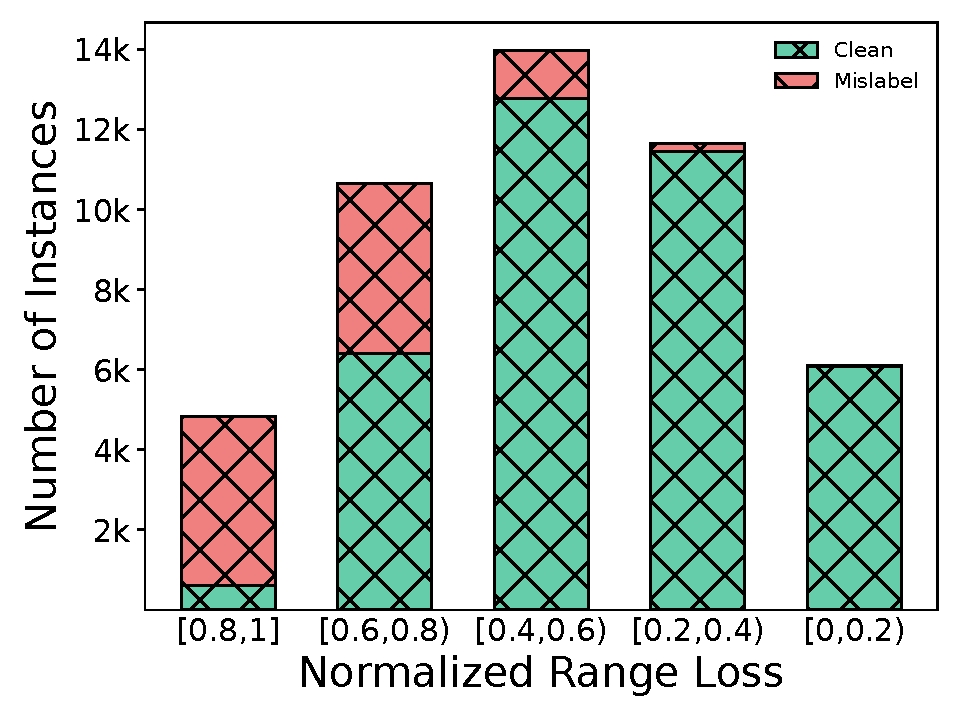
\includegraphics[width=0.35\textwidth]{figures/loss}
	\caption{An Example of Early Loss.}
	\label{fig:loss}
\end{figure}

Therefore,  we observed that the \textit{early loss} can well distinguish mislabeled instances from clean ones. Early loss means the loss of each instance at early training epochs. As shown in Figure~\ref{fig:loss}, the X-axis denotes the range of normalized loss after training the first epoch,  and the Y-axis denotes the number of instances falling into the corresponding range. We can see that  the mislabeled instances always have large loss, while the clean ones are associated with relatively small loss. 

\stitle{Our proposal.} Based on the above observation, generally speaking, we can conclude that mislabeled instances are harder for an ML model to fit than the clean instances especially at early epochs, leading to large loss. Therefore, we propose our \sys framework that leverages the early loss to detect mislabeled instances in an ML training set. The key idea is straightforward yet effective that at each early epoch,  we sort the instances in the training set according to the loss in descending order. Then we tend to iteratively identify top instances as mislabeled ones and remove them from the training set. We remove because we hope to  navigate the model  towards a well-performed one, as if it is trained over clean instances. In this way, at the subsequent epochs, the model can better fit clean instances and recognize mislabeled ones. 

However, to make the model better, purely removing instances with the largest value is sub-optimal because an instance with a large loss does not imply it has a large impact on the model. Hence, \sys has another module  to estimate the influence of each instance. A higher influence indicates that if we identify the corresponding instance as mislabeled and remove it, the model will be more affected and quickly lead to a well-performed model trained over clean instances. Besides, we also design a strategy to estimate the rate of mislabeled instances, so as to help judge when the \sys stops. What's more, there are likely to  exist some outliers in each dataset, which are also hard to be  fitted by a model at early epochs with large loss. If they are identified as mislabeled, our precision goes down. Hence, we also propose a module to cope with these outliers.


\stitle{Contributions.}
Our contributions are summarized as follows:

\noindent (1) We formally model the mislabel detection problem and  design an iterative mislabel detection framework \sys with high accuracy based on machine learning training.

\noindent (2) We introduce the early loss to help determine whether an instance is mislabeled, which is very effective.

\noindent (3) We propose an influence computation method customized to our problem to further improve the performance of  mislabel detection, based on the influence function. 

\noindent (4) Sufficient experiments on XX datasets over XX baselines demonstrate that \sys outperforms them up to XX in terms of the F1-score.

\begin{figure*}
	\centering
	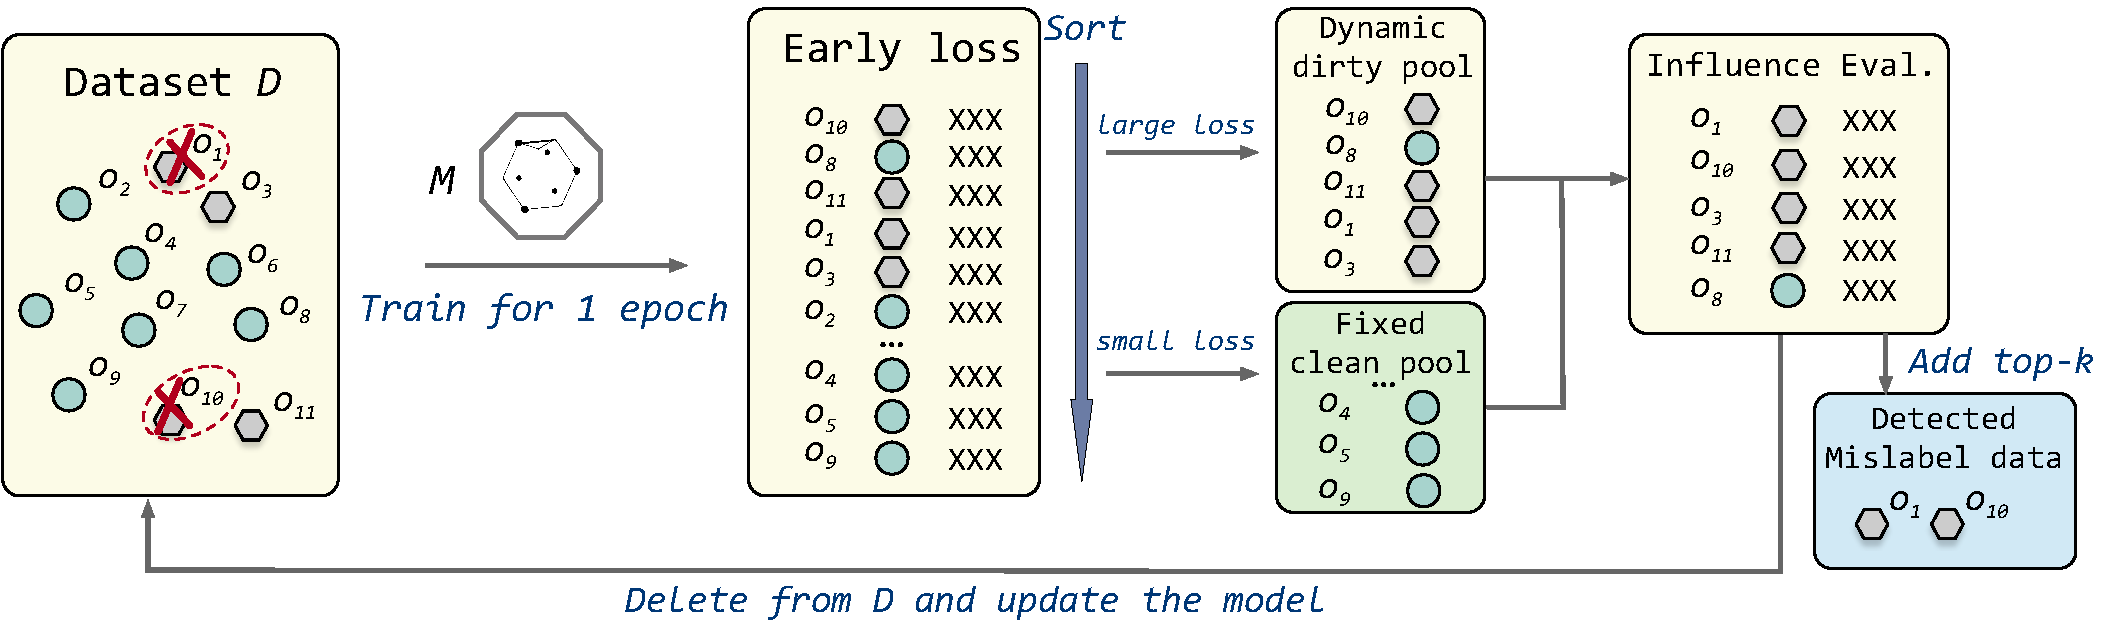
\includegraphics[width=\textwidth]{figures/framework}
	\caption{\sys Framework}
	\label{fig:framework}
\end{figure*}

The paper is organized as follows. We first introduce the preliminaries including the problem definition in Section~\ref{sec:pre}. Then the overall framework is introduced in  Section~\ref{sec:framework}. Next, we introduce the details of how to use early loss to detect mislabels (Section~\ref{sec:loss}), followed by using the instance influence to further improve the performance Section~\ref{sec:incluence}. Furthermore, we design other optimization techniques like mislabel rate estimation, and outlier processing in Section~\ref{sec:outlier}. Related work is discusses in Section~\ref{sec:related} and we conduct experiments in Section~\ref{sec:exp}. The significant notations used in this paper are listed in Table~\ref{tab:notation}.


\begin{table}
	\centering
	\caption{Notation Table}
	\vspace{-1em}
	{
		\begin{tabular}{|c|c|}
			\hline
			{\bf Notations} & {\bf Description}  \\
			\hline	
			$\train$ & Entire train set including mislabeled instances. \\\hline
			$\train_m$ & The set of mislabeled instances ($\train_m \subseteq \train$).   \\\hline			
			$\train_c$ & The set of clean instances ($ \train = \train_m \cup \train_c $).  \\\hline
			$\model$ & Downstream model for mislabel detection.   \\\hline
			$\model$ & Downstream model for mislabel detection.   \\\hline
			$\model$ & Downstream model for mislabel detection.   \\\hline
			$\model$ & Downstream model for mislabel detection.   \\\hline
			$\model$ & Downstream model for mislabel detection.   \\\hline	
		\end{tabular}
	}
	\label{tbl:dataset}
	\vspace{-2.2em}
\end{table}


% \begin{figure*}
%	\centering
%	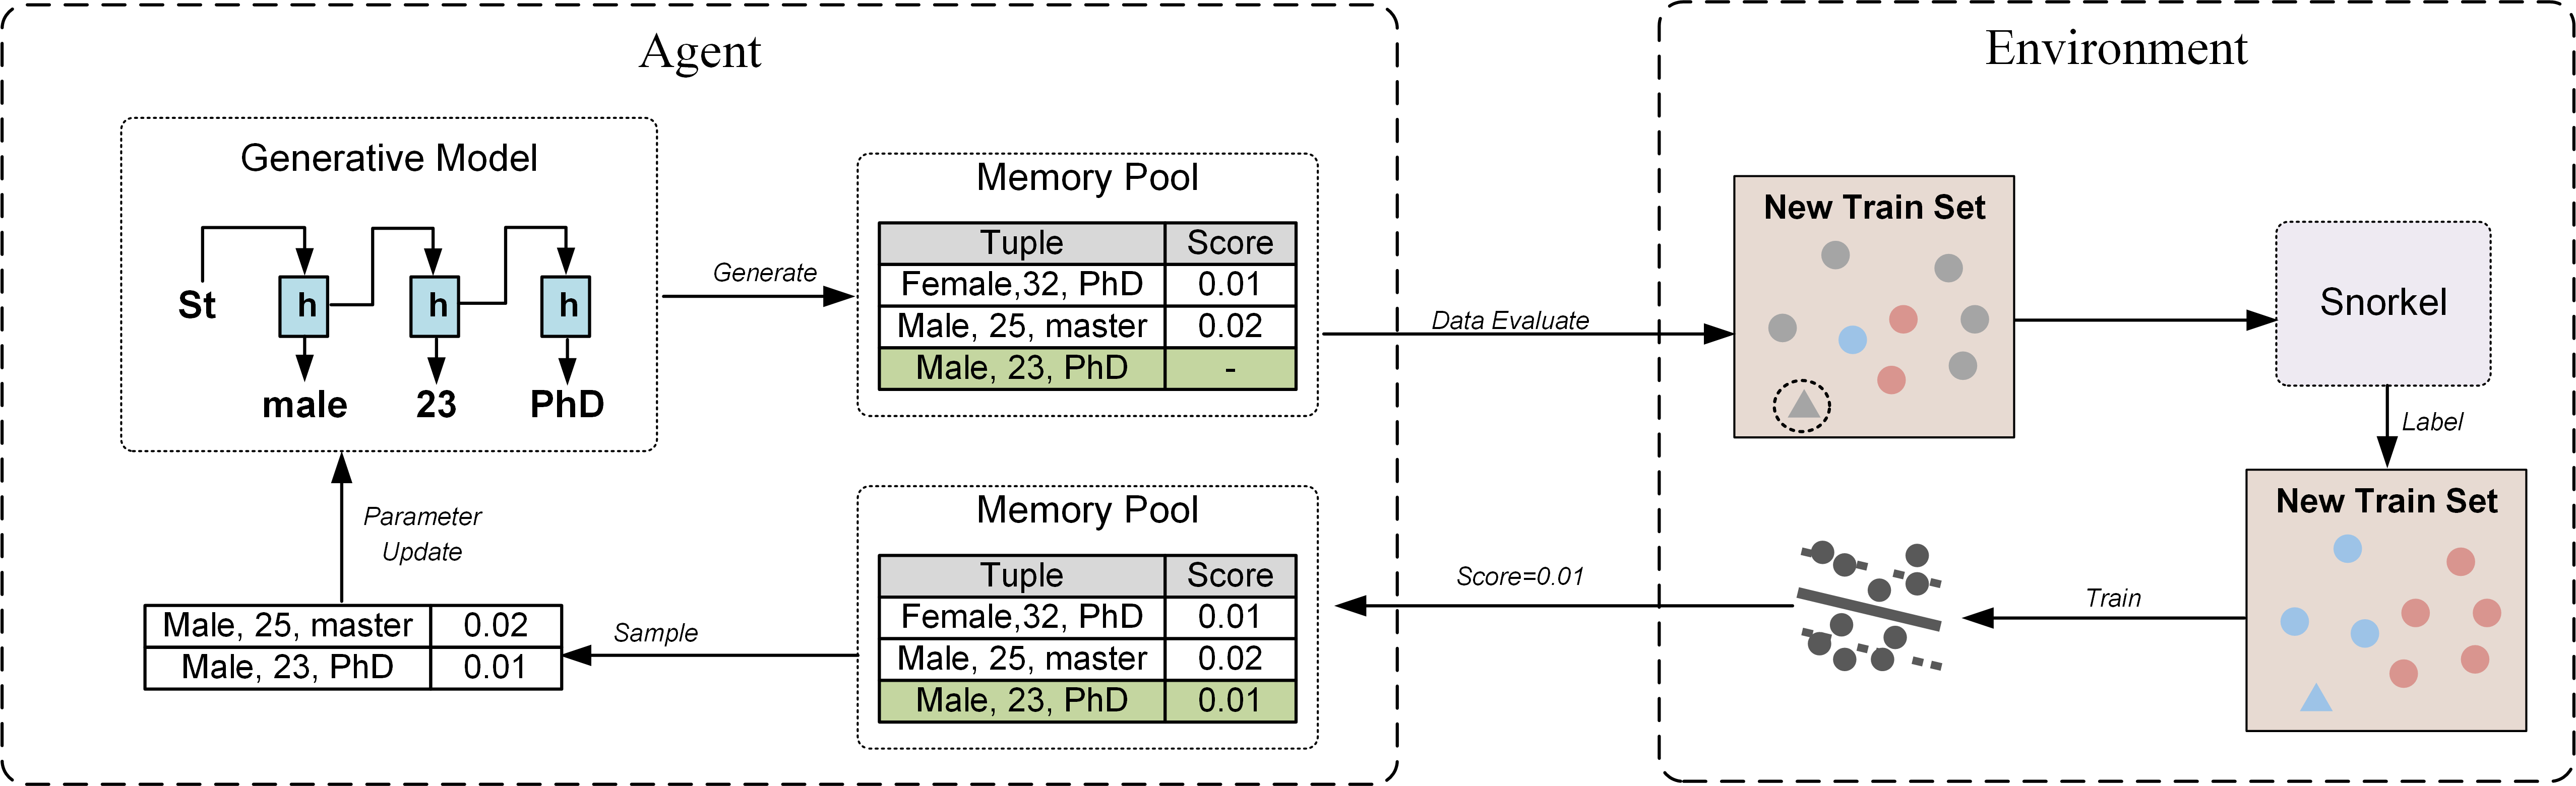
\includegraphics[width=\textwidth]{figures/overview.png}
%	\caption{Framework}
%	\label{fig:framework}
% \end{figure*}

% \begin{itemize}
% 	\item The difference between traditional data generation and ours (for ML model).
% 	\item (Challenge) The key challenges of this problem: learn the generative model from feedback; how to evaluate generated tuples.
% \end{itemize}